\documentclass[11pt]{article}
\usepackage[margin=1in]{geometry}
\usepackage{mathpazo}
\usepackage{amsmath,amssymb}
\usepackage{microtype}
\usepackage{booktabs}
\usepackage{graphicx}
\usepackage[dvipsnames]{xcolor}
\usepackage{tikz}
\usetikzlibrary{positioning,arrows.meta,calc,fit,backgrounds}
\usepackage[most]{tcolorbox}
\usepackage{enumitem}
\usepackage{listings}
\usepackage[font=small,labelfont=bf]{caption}
\usepackage{hyperref}
\hypersetup{colorlinks=true,linkcolor=MidnightBlue,citecolor=MidnightBlue,urlcolor=MidnightBlue}
\usepackage{cleveref}
\urlstyle{tt}
\def\UrlBreaks{\do\_\do/\do.}
\newcommand{\file}[1]{\nolinkurl{#1}}
\newcommand{\code}[1]{\texttt{#1}}
\newcommand{\mhh}{m_{hh}}
\newcommand{\bw}{\boldsymbol{\omega}}
\newcommand{\bp}{\boldsymbol{p}}
\newcommand{\bx}{\boldsymbol{x}}
\newcommand{\data}{\mathcal{D}}

\definecolor{trainable}{HTML}{1B6CA8}
\definecolor{physics}{HTML}{2E933C}
\definecolor{datac}{HTML}{7B4EA3}
\definecolor{warn}{HTML}{C0392B}

\newtcolorbox{keyidea}[1][]{enhanced,breakable,colback=physics!6,colframe=physics!70!black,
  fonttitle=\bfseries,title={#1},boxrule=0.6pt,arc=2pt,left=6pt,right=6pt}
\newtcolorbox{aside}[1][]{enhanced,breakable,colback=trainable!5,colframe=trainable!70!black,
  fonttitle=\bfseries,title={#1},boxrule=0.6pt,arc=2pt,left=6pt,right=6pt}
\newtcolorbox{assume}[1][]{enhanced,breakable,colback=datac!5,colframe=datac!70!black,
  fonttitle=\bfseries,title={#1},boxrule=0.6pt,arc=2pt,left=6pt,right=6pt}
\newtcolorbox{watch}[1][]{enhanced,breakable,colback=warn!5,colframe=warn!70!black,
  fonttitle=\bfseries,title={#1},boxrule=0.6pt,arc=2pt,left=6pt,right=6pt}
\setlist{itemsep=2pt,topsep=3pt}
\setlength{\emergencystretch}{3em}

\lstset{language=Python, basicstyle=\ttfamily\small, columns=fullflexible,
  keepspaces=true, commentstyle=\color{physics!70!black}\itshape,
  keywordstyle=\color{trainable!90!black}\bfseries, stringstyle=\color{datac},
  showstringspaces=false, frame=single, rulecolor=\color{gray!40},
  backgroundcolor=\color{gray!3}, xleftmargin=4pt, xrightmargin=4pt,
  aboveskip=6pt, belowskip=6pt}

\title{\textbf{The first Bayesian neural network for \texttt{dihiggs}}\\[4pt]
\large Results of the run \texttt{runs/BNN\_laplace} on the RTX 5090}
\date{October 30, 2026}

\begin{document}
\maketitle

\begin{abstract}
\noindent
The notebook \file{heft_train_bnn.ipynb} was run with its default settings on an
RTX~5090: Laplace likelihood, warm start from \file{runs/L1Loss}, 500 warm-up
iterations, 1,000 saved samples, 100 leapfrog steps per trajectory, one chain. It took
about 10 minutes. This note examines the result; \cref{sec:mixing} recalls what the convergence
diagnostics used here mean. The sampler itself works as intended:
the acceptance rate is on target, there are no divergences, and the energy, the noise
scale and the 16 prior precisions mix well. The predictions of the network, however,
do not: at one of the two monitored points the chain drifts, with an effective sample
size of about 5. The credible bands are about fifty times narrower than the POWHEG
noise and contain only 4\% of the holdout POWHEG values at 95\% credibility; they
describe one narrow valley of the posterior, not the real error of the model. A
welcome by-product is that the sampled networks fit the holdout spectra better than
the warm-start model, especially near threshold, where the mean $\chi^2$ per bin
falls from 8.4 to 3.6. Four changes for the next runs are recommended in
\cref{sec:next}.
\end{abstract}

\begin{keyidea}[The main findings]
\begin{enumerate}
  \item \textbf{The sampler is healthy.} Acceptance 0.84 (target 0.8), no divergences
    after warm-up; $U$, $b$ and all $\tau_g$ have effective sample sizes of 600--1,000
    out of 1,000 and split-$\hat R \approx 1.00$.
  \item \textbf{The predictions are not converged.} The Standard Model prediction at
    997.5~GeV drifts (effective sample size 5, split-$\hat R = 1.54$). The likely
    cause: each trajectory moves only about 0.4 posterior standard deviations.
  \item \textbf{The bands are far too narrow to be an error on the model.} Their width
    is typically 2\% of the POWHEG noise, while the model's actual error is about 36\%
    of it. They measure parameter uncertainty in one valley, assuming the model is
    right; they do not measure how far the model is from POWHEG.
  \item \textbf{The fit improved.} Median $\chi^2/N$ on the holdout spectra 1.17
    $\to$ 1.13; spectra with $\chi^2/N > 5$ 4.9\% $\to$ 2.5\%; mean $\chi^2$ per bin
    at 255--555~GeV 8.4 $\to$ 3.6; negative predictions 0.18\% $\to$ 0.07\%. The gain
    comes from the first few trajectories, not from averaging.
\end{enumerate}
\end{keyidea}

\tableofcontents

% ===========================================================================
\section{The run}

\begin{center}
\small
\begin{tabular}{ll}
\toprule
setting & value\\
\midrule
likelihood & Laplace, scale $b$ Gibbs-sampled\\
prior & Neal's hierarchical prior, 16 groups, $\tau_g$ Gibbs-sampled\\
warm start & \file{runs/L1Loss/dihiggs_params.pth}\\
training rows & 274,152 (all), every gradient over all of them\\
iterations & 500 warm-up + 1,000 saved ($\code{THIN} = 1$)\\
leapfrog steps & $L = 100$ (jittered by $\pm 10\%$)\\
chains & 1, seed 42\\
time & about 10 minutes on an RTX 5090\\
\bottomrule
\end{tabular}
\end{center}

\noindent The 1,000 sampled parameter sets were evaluated with \code{hmc.BNN} on all
1,000 holdout spectra ($80{,}000$ bins). For $\chi^2$, the POWHEG noise of each bin is
estimated as in \file{heft_test.ipynb}, $\sigma_k^2 = f_k\,\sigma_\text{tot}/N_\text{eff}$
with $N_\text{eff} = 38{,}024$, for bins with $f_k > 0$.

% ===========================================================================
\section{A reminder: mixing and how it is diagnosed}
\label{sec:mixing}

\paragraph{What mixing means.} A Markov chain produces a sequence of parameter sets
$\bw_1, \bw_2, \ldots$, each obtained from the one before. \emph{Mixing} describes how
quickly the chain forgets where it has been and explores the whole posterior. In a
well-mixed chain, samples a few iterations apart are nearly independent draws from the
posterior. In a poorly mixed chain, each sample is almost a copy of the previous one, so
that 1,000 samples carry the information of only a handful. Mixing is a property of each
quantity separately: a chain can explore some directions in parameter space quickly and
others slowly, and in this run it did exactly that.

\paragraph{1. Trace plots.} Plot a quantity against the iteration number. A well-mixed
chain looks like a ``fuzzy caterpillar'': rapid fluctuations about a constant level, as
$U$ and $b$ do in \cref{fig:traces}. A poorly mixed chain wanders, with long excursions
and trends, like the 997.5~GeV prediction in the same figure.

\paragraph{2. Autocorrelation.} The autocorrelation at lag $k$, $\rho(k)$, is the
correlation between a quantity at iteration $i$ and at iteration $i + k$, averaged over
$i$. For a well-mixed quantity it falls to zero within a few lags; for a poorly mixed one
it stays positive for many lags: the chain still ``remembers'' where it was
(\cref{fig:acf}).

\paragraph{3. Effective sample size.} The autocorrelations are combined into the number
of \emph{independent} draws that would give the same precision:
\begin{equation}
  n_\text{eff} = \frac{N}{1 + 2\sum_{k \ge 1} \rho(k)} ,
  \label{eq:ess}
\end{equation}
where $N$ is the number of samples. The denominator, the \emph{integrated autocorrelation
time}, is roughly the number of iterations needed to obtain one independent draw. (In
practice the sum is stopped when the autocorrelations become indistinguishable from
noise; \code{hmc.ess} uses Geyer's rule, stopping at the first negative sum of a pair of
consecutive autocorrelations.) What $n_\text{eff}$ is for: the Monte Carlo error of a
posterior mean is
\[
  \frac{\text{posterior standard deviation}}{\sqrt{n_\text{eff}}}
  \qquad\text{and not}\qquad
  \frac{\text{posterior standard deviation}}{\sqrt{N}} .
\]

\paragraph{4. $\hat R$, the Gelman--Rubin statistic.} Run several chains (or split one
chain into halves) and compare the variance \emph{between} them, $B$, with the average
variance \emph{within} each, $W$:
\begin{equation}
  \hat R = \sqrt{\frac{\tfrac{n-1}{n}\,W + \tfrac{1}{n}\,B}{W}} ,
  \label{eq:rhat}
\end{equation}
where $n$ is the length of each chain and $B$ is $n$ times the variance of the chain
means. If every chain, or every part of one chain, has sampled the same distribution, the
chain means agree to within their Monte Carlo errors and $\hat R \approx 1$. Values above
about 1.05 mean the parts disagree: the chain is still moving or the chains are in
different places.

\begin{keyidea}[What the diagnostics showed in this run]
\begin{center}
\small
\begin{tabular}{lccc}
\toprule
quantity & trace & $\rho$ at lag 300 & $n_\text{eff}$ (of 1,000), split-$\hat R$\\
\midrule
$U$, $b$, $\tau_g$ & caterpillar & $\approx 0$ & 600--1,070, 1.00\\
SM prediction, 262.5 GeV & caterpillar & $\approx 0$ & 123, 1.02\\
SM prediction, 997.5 GeV & wanders, then drifts down & $\approx 0.1$ & \textbf{5}, \textbf{1.54}\\
\bottomrule
\end{tabular}
\end{center}
The chain was not frozen: 84\% of the trajectories were accepted, and most quantities
moved freely. One direction in parameter space, the one that controls the high-mass
prediction, was explored only by a slow random walk. With $n_\text{eff} = 5$, the
posterior mean of that prediction is known only to about $1/\sqrt{5} \approx 0.45$
posterior standard deviations, and its posterior standard deviation is itself unreliable,
because a slowly wandering chain has not yet covered the full width of the distribution.
\end{keyidea}

\paragraph{Why some directions mix and others do not.} Each trajectory moves the
parameters a distance of about $\varepsilon L$ in units of their posterior standard
deviations (\cref{sec:sampler}). In directions where the posterior is narrow, a move of
0.4 standard deviations is enough to decorrelate successive samples. In a long, flat
direction it is not: successive trajectories point in random directions, and a random walk
of step $\delta$ needs about $(D/\delta)^2$ steps to cover a distance $D$. To cross
10 standard deviations in steps of 0.4 takes about 600 iterations, longer than the run.
HMC was invented to avoid exactly this: with trajectories long enough, it crosses the
posterior in a straight line instead of diffusing across it (\file{bnn_plan.pdf},
Fig.~1). Hence the first recommendation of \cref{sec:next}.

\begin{watch}[What none of these diagnostics can show]
Every diagnostic above measures how well the chain has explored the region it is in.
A single chain can mix perfectly within one valley of a posterior with several valleys,
and never find the others; its trace plots, autocorrelations and split-$\hat R$ will all
look fine. The main protection is to run several chains from different starting points
and compute $\hat R$ \emph{across} them. With every chain warm-started from the same
L1 model, even that tests only whether they leave the same valley in the same way;
chains started from different trained models would be a stronger test.
\end{watch}

% ===========================================================================
\section{The sampler}
\label{sec:sampler}

\begin{figure}[h]
\centering
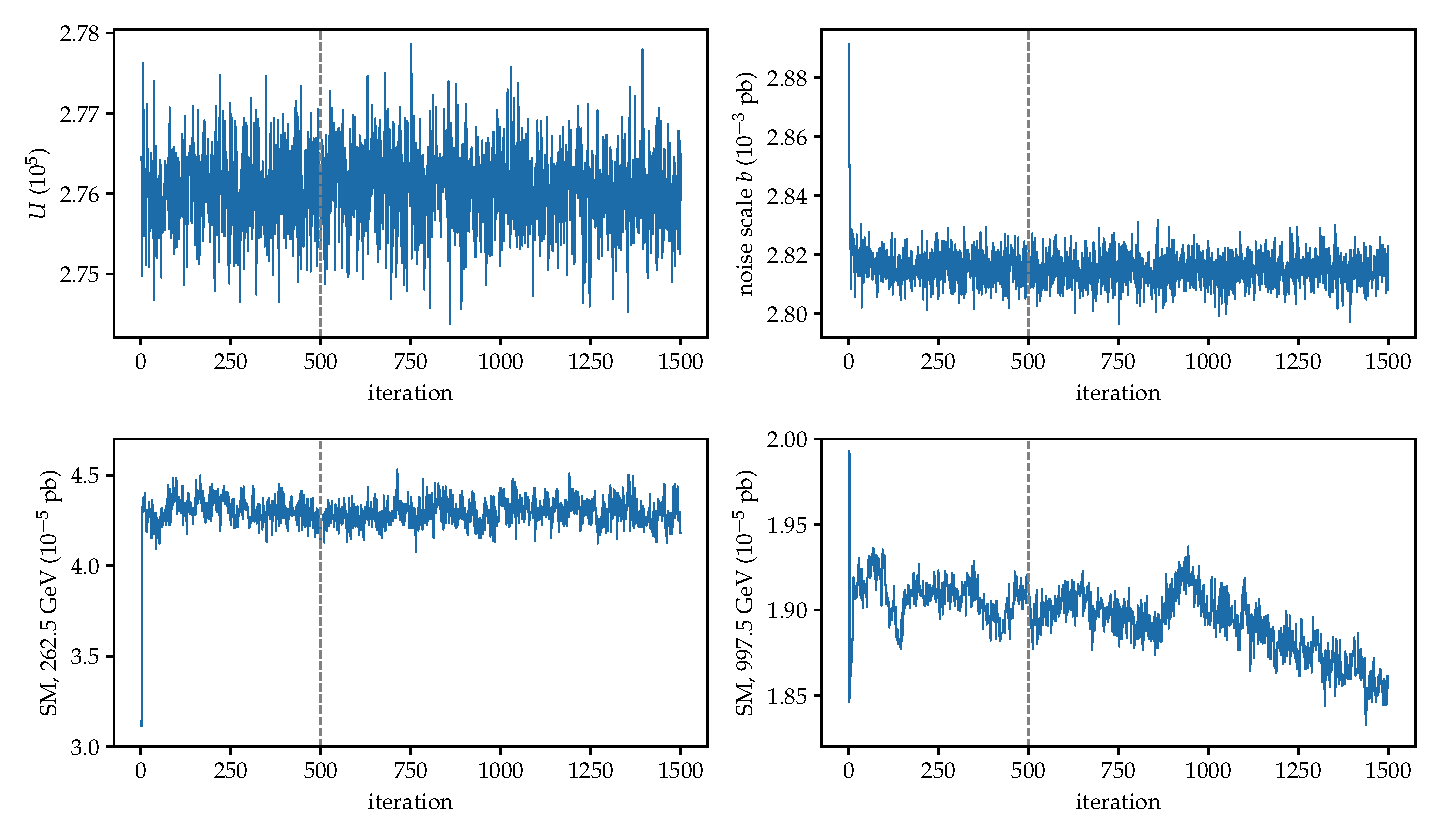
\includegraphics[width=\textwidth]{fig_traces.pdf}
\caption{Traces of the potential energy $U$, the noise scale $b$, and the two monitor
values: the predictions for the Standard Model point
$(\kappa_\lambda, c_t, c_{tt}, c_{ggh}, c_{gghh}) = (1, 1, 0, 0, 0)$ in the first bin
above threshold and in the bin at 997.5~GeV. The dashed line marks the end of the
warm-up. Note the jump of the 262.5~GeV prediction in the first few iterations, and the
drift of the 997.5~GeV prediction.}
\label{fig:traces}
\end{figure}

\begin{center}
\small
\begin{tabular}{lrrr}
\toprule
quantity & effective sample size (of 1,000) & split-$\hat R$ & verdict\\
\midrule
$U$ & 979 & 1.002 & mixes well\\
noise scale $b$ & 1,005 & 0.999 & mixes well\\
$\tau_1, \ldots, \tau_{16}$ & 625--1,070 & 0.999--1.008 & mix well\\
SM prediction, 262.5 GeV & 123 & 1.015 & adequate\\
SM prediction, 997.5 GeV & 5 & 1.538 & \textbf{not converged}\\
\bottomrule
\end{tabular}
\end{center}

\noindent The acceptance rate was 0.78 during warm-up and 0.84 afterwards. There were
four divergences, all in the first few iterations of the warm-up, while the step size was
still being found, and none afterwards. $U$ and $b$ show no trend, and $b$ settles at
$2.815 \times 10^{-3}$~pb, the mean absolute residual, as it should for a Laplace
likelihood.

\begin{aside}[Split-$\hat R$]
With a single chain, $\hat R$ is computed by splitting the 1,000 samples into two halves
and treating them as two chains. A value well above 1 means the two halves describe
different distributions, i.e.\ the chain is still moving.
\end{aside}

\Cref{fig:acf} shows why the two kinds of quantity differ. The autocorrelation of $U$,
$b$ and the 262.5~GeV prediction falls to zero within a few iterations; that of the
997.5~GeV prediction is still 0.1 after 300 iterations. The chain therefore explores
the directions that control $U$ and $b$ quickly, but some direction in parameter space
that moves the high-mass prediction only very slowly, by a random walk.

\begin{figure}[h]
\centering
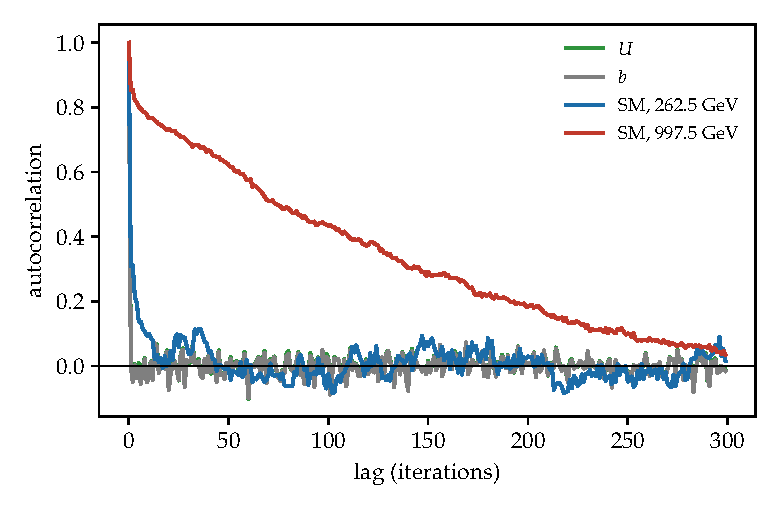
\includegraphics[width=0.6\textwidth]{fig_acf.pdf}
\caption{Autocorrelation after warm-up as a function of the lag.}
\label{fig:acf}
\end{figure}

\begin{watch}[Why the chain is slow: trajectories that are too short]
After warm-up the step size is $\varepsilon \approx 0.0044$ in the units set by the
mass matrix, in which each parameter's posterior standard deviation is about 1. With
$L = 100$ steps, a trajectory lasts $\varepsilon L \approx 0.44$, so it moves each
parameter by less than half a standard deviation. HMC's advantage over a random walk
comes from trajectories long enough to cross the posterior (\file{bnn_plan.pdf},
Fig.~1); here they are not. A second likely contributor is the mass matrix itself,
estimated from iterations 75--425 of warm-up, a stretch over which the slow directions
barely moved, so their variance, and hence the step allowed along them, is
underestimated.
\end{watch}

% ===========================================================================
\section{The jump at the start}
\label{sec:jump}

The first two trajectories were rejected (the step-size search was still under way).
The next three were accepted with energy changes $\Delta H = -78$, $-58$ and $-13$,
and in those three trajectories the Standard Model prediction at 262.5~GeV rose from
$3.11 \times 10^{-5}$ to $4.37 \times 10^{-5}$~pb, by 40\%. It then stayed within
$\pm 1.6\%$ of $4.29 \times 10^{-5}$~pb for the rest of the run.

Two things follow. First, the warm-start model was not at the top of the posterior: a
direction existed in which $U$ fell quickly, and the first trajectories followed it.
Second, near threshold the prediction for a given $\theta$ is so weakly constrained that
a small move of the parameters changed it by 40\% at no cost in fit quality. The
posterior band of $\pm 1.6\%$ found afterwards is the width of the valley the chain
landed in, not the uncertainty on the prediction.

% ===========================================================================
\section{Comparison with the holdout spectra}
\label{sec:holdout}

\begin{center}
\small
\begin{tabular}{lcccc}
\toprule
model & median $\chi^2/N$ & $\chi^2/N > 2$ & $\chi^2/N > 5$ & negative predictions\\
\midrule
\file{L1Loss} (warm start) & 1.171 & 13.6\% & 4.9\% & 0.18\%\\
BNN posterior mean & 1.127 & 9.2\% & 2.5\% & 0.07\%\\
BNN, first sample & 1.134 & 9.2\% & 2.5\% & \\
BNN, last sample & 1.131 & 9.3\% & 2.4\% & \\
\bottomrule
\end{tabular}
\end{center}

\noindent The improvement is concentrated near threshold (\cref{fig:holdout}a): the mean
$\chi^2$ per bin between 255 and 555~GeV falls from 8.4 to 3.6, and above 555~GeV from
1.20 to 1.16. Every individual sample is as good as the mean, so the gain is not an
averaging effect. It comes from the move of \cref{sec:jump}.

\begin{keyidea}[A plausible explanation, worth testing]
The Laplace posterior's most probable point is full-batch L1 training with a little
weight decay (\file{bnn_plan.pdf}, \S2.3). The warm start came from mini-batch Adam,
which stops at a noisy point. The first HMC trajectories, which use exact full-data
gradients, completed the optimisation. If so, a short full-batch L1 fine-tune of the
trained model, with weight decay, would give the same improvement without HMC, and
\file{heft_train.ipynb} could gain it cheaply.
\end{keyidea}

\begin{figure}[h]
\centering
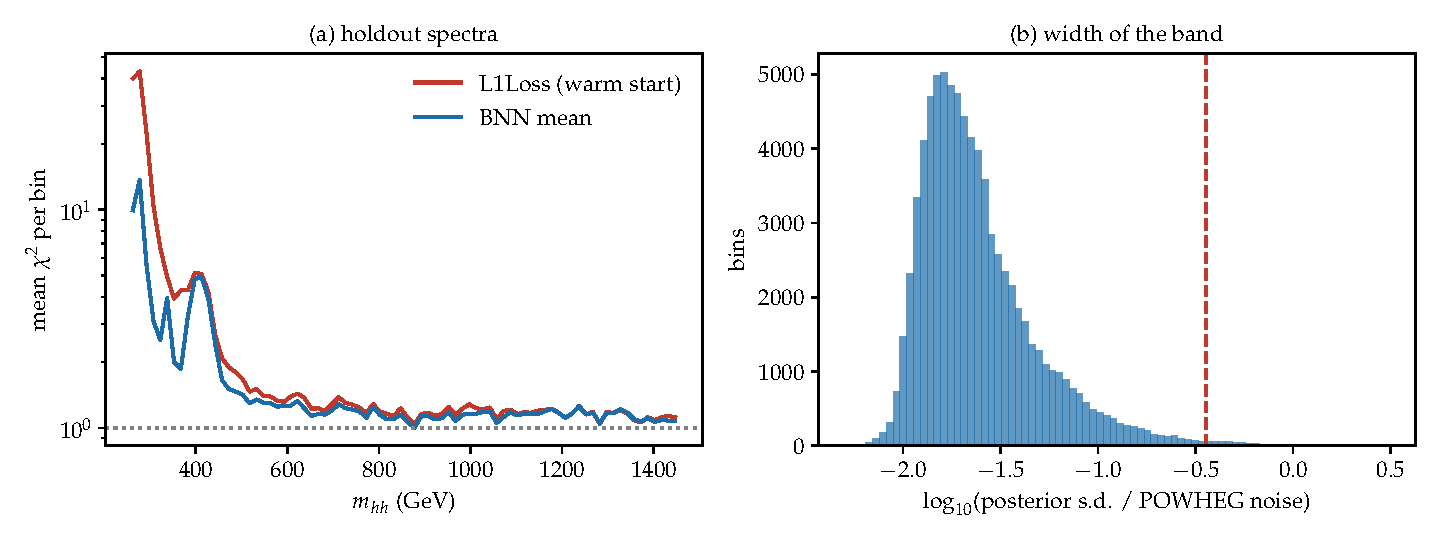
\includegraphics[width=\textwidth]{fig_holdout.pdf}
\caption{(a) Mean $\chi^2$ per bin over the 1,000 holdout spectra, against $\mhh$, for the
warm-start model and the BNN mean. (b) Distribution over all holdout bins of the
posterior standard deviation divided by the POWHEG noise $\sigma_k$. The dashed line,
at 0.36, is the model's typical actual error in the same units,
$\sqrt{\chi^2/N - 1}$ with $\chi^2/N = 1.13$.}
\label{fig:holdout}
\end{figure}

% ===========================================================================
\section{How wide are the bands?}
\label{sec:bands}

\begin{itemize}
  \item The posterior standard deviation of a bin is typically \textbf{2\%} of the
    POWHEG noise (median 0.021; 90\% of bins below 0.063; 99\% below 0.28;
    \cref{fig:holdout}b). It is only a little larger near threshold (median 0.026) than
    elsewhere (0.020).
  \item The model's actual error is about \textbf{36\%} of the noise. The band is
    therefore about 17 times narrower than the error it would need to describe.
  \item Only \textbf{4.2\%} of the holdout POWHEG values lie inside the 95\% credible band.
    Part of that is expected, since the band is for the true function and POWHEG values
    contain noise. But the band is also far narrower than the model's own error, so
    even noise-free POWHEG values would mostly fall outside it.
  \item The BNN mean differs from the warm-start model by a median of \textbf{5}
    posterior standard deviations (90\% of bins: under 13), although the two are
    equally plausible fits.
  \item The means of the first and the second 500 samples differ by a median of
    \textbf{0.5} posterior standard deviations: the band is still moving, as the
    997.5~GeV trace showed.
\end{itemize}

\begin{assume}[What the band does and does not mean]
A Bayesian credible band is the uncertainty on the function \emph{if the model and the
likelihood are correct}. With 274,000 rows the parameters of a 3,944-parameter network
are tightly constrained, so a narrow band is not in itself wrong. Three things make this
one narrower than the real uncertainty:
\begin{enumerate}
  \item \textbf{Incomplete exploration.} The chain has not yet explored even the valley
    it is in (\cref{sec:sampler}).
  \item \textbf{Several valleys.} Networks that fit equally well but differ in the
    sparsely constrained regions (\cref{sec:jump}) lie in different valleys. One chain
    sees one of them.
  \item \textbf{A misspecified model.} The model's systematic error near threshold
    (mean $\chi^2$ per bin 3.6) is not described by any parameter spread. Neither is
    the noise: the Laplace scale $b = 2.8 \times 10^{-3}$~pb is the same for a
    $10^{-5}$~pb bin and a 1~pb bin.
\end{enumerate}
\end{assume}

% ===========================================================================
\section{Recommendations for the next runs}
\label{sec:next}

\begin{enumerate}
  \item \textbf{Longer trajectories:} \code{N\_LEAPFROG} = 500--1,000, so that each
    trajectory lasts $\varepsilon L$ = 2--4 standard deviations. Cost: 5--10 times
    the present run, i.e.\ about 50--100 minutes.
  \item \textbf{A longer warm-up:} \code{N\_WARMUP} = 1,000, for a better mass matrix
    and so a larger step size.
  \item \textbf{Four chains:} \code{N\_CHAINS} = 4. The spread between chains in the
    monitored predictions, and $\hat R$ across chains, will show whether different
    chains settle in different valleys. I expect they will, and that the spread is
    closer to the model's real uncertainty.
  \item \textbf{The \code{'poisson'} likelihood,} to obtain bands whose width can be
    compared with POWHEG bin by bin. It is experimental: the corresponding CHI2 loss
    trained poorly, although with a warm start the sampler does not have to find the
    minimum from scratch.
\end{enumerate}

\noindent The first of these is now being tested: a run with the \code{'poisson'}
likelihood, \code{N\_WARMUP} = 1,500, \code{N\_SAMPLES} = 500, \code{N\_LEAPFROG} = 500
and one chain. Because the L1 starting point is far from the $\chi^2$ optimum
(the energy fell by 20\% within 80 iterations in a test on 80 spectra), the first thing
to check is that $U$ has levelled off well before the end of the warm-up; otherwise the
mass matrix is estimated from the descent rather than from the posterior.

\noindent What to look at in each new run: the effective sample size and split-$\hat R$ of
\code{m\_1}; for several chains, $\hat R$ across chains and the chain-to-chain spread
of the monitored predictions compared with the within-chain spread; and, on the
holdout spectra, the fraction of POWHEG values inside the predictive band.

\paragraph{Separately, worth testing.} A full-batch L1 fine-tune of the trained model
with weight decay (\cref{sec:holdout}), to see whether it reproduces the improvement at
threshold without HMC.

\paragraph{A plotting fault.} In the relative-band panels of
\file{dihiggs_spectra_bands.png}, a single bin near threshold sometimes sets the vertical
range and hides the rest of the band (e.g.\ the last spectrum). The fix is to limit the
range to, say, the 2nd to 98th percentile of the plotted values. It is not yet made, so
as not to change the notebook while it is running.

\end{document}
